%% 
%% Copyright 2019-2020 Elsevier Ltd
%% 
%% This file is part of the 'CAS Bundle'.
%% --------------------------------------
%% 
%% It may be distributed under the conditions of the LaTeX Project Public
%% License, either version 1.2 of this license or (at your option) any
%% later version.  The latest version of this license is in
%%    http://www.latex-project.org/lppl.txt
%% and version 1.2 or later is part of all distributions of LaTeX
%% version 1999/12/01 or later.
%% 
%% The list of all files belonging to the 'CAS Bundle' is
%% given in the file `manifest.txt'.
%% 
%% Template article for cas-dc documentclass for 
%% double column output.

\documentclass[a4paper,fleqn]{cas-dc}
\usepackage[authoryear,longnamesfirst]{natbib}


\begin{document}
\let\WriteBookmarks\relax
\def\floatpagepagefraction{1}
\def\textpagefraction{.001}

\shorttitle{Analiza zbioru pacjętów z SM chorych na COVID-19 modelem One-CLass SVM}

\shortauthors{}

\title [mode = title]{Analiza zbioru danych "Patient-level dataset to study the effect of COVID-19 in people with Multiple Sclerosis" z wykorzystaniem nadzorowanego algorytmu uczenia maszynowego One-Class SVM(Support Vector Machines)}                      

\author{Anna Mrozek, Bartosz Panek \,i\, Przemysław Jura  }

\renewcommand{\abstractname}{STRESZCZENIE}
\begin{abstract}
Artykuł analizuje zbiór danych pacjentów ze stwardnieniem rozsianym (SM), którzy przeszli COVID-19, przy użyciu nadzorowanego algorytmu One-Class SVM. Celem jest identyfikacja przypadków o zwiększonym ryzyku ciężkiego przebiegu infekcji. Umożliwi to zidentyfikowanie charakterystycznych cech pacjentów bardziej narażonych na powikłania.
\end{abstract}

\renewcommand{\abstractname}{STRESZCZENIE}
\begin{keywords}
One-Class SVM \sep COVID-19 
\end{keywords}

\maketitle

\section{Wprowadzenie}
Pandemia COVID-19 miała znaczący wpływ na osoby z chorobami przewlekłymi, w tym na pacjentów ze stwardnieniem rozsianym (SM). SM jest przewlekłą chorobą autoimmunologiczną, która wpływa na układ nerwowy i może prowadzić do trwałego uszkodzenia neuronów oraz ograniczenia funkcji motorycznych oraz poznawczych.[1][2] Ze względu na charakter choroby i stosowane terapie immunosupresyjne, pacjenci z SM mogą być bardziej narażeni na cięższy przebieg infekcji wirusowych, w tym COVID-19.[3][4] Analiza danych od pacjentów z SM, którzy przeszli COVID-19, może dostarczyć ważnych informacji na temat ryzyka powikłań i zidentyfikować czynniki przyczyniające się do poważniejszych objawów, co ostatecznie może pomóc w lepszym monitorowaniu i opiece nad tą grupą pacjentów.

\section{Cel}
Celem badania jest wykorzystanie nadzorowanego algorytmu One-Class SVM do analizy zbioru danych pacjentów ze stwardnieniem rozsianym, którzy przeszli COVID-19, w celu zidentyfikowania cech pacjentów o zwiększonym ryzyku ciężkiej infekcji. Oczekuje się, że wyniki analizy dostarczą wskazówek do opracowania bardziej ukierunkowanych strategii opieki i środków zapobiegawczych dla pacjentów ze stwardnieniem rozsianym w kontekście potencjalnych przyszłych pandemii lub innych zagrożeń wirusowych.

\section{Przegląd literatry}
W literaturze medycznej i naukowej, od początku pandemii COVID-19, wiele badań skupiało się na analizie wpływu wirusa SARS-CoV-2 na osoby cierpiące na choroby przewlekłe i autoimmunologiczne, takie jak stwardnienie rozsiane (SM). Wyniki tych badań sugerują, że pacjenci z SM, zwłaszcza ci stosujący terapie immunosupresyjne, mogą być bardziej narażeni na cięższy przebieg COVID-19 oraz związane z nim powikłania[5][6]. U pacjentów z SM często obserwuje się obniżoną odporność oraz większą podatność na infekcje, co wynika zarówno z samej choroby, jak i z efektów leków tłumiących układ odpornościowy[7]. Dodatkowo w badaniach zwraca się uwagę na takie czynniki ryzyka jak wiek, płeć, rodzaj stosowanego leczenia oraz inne choroby towarzyszące, które mogą zwiększać ryzyko ciężkiego przebiegu infekcji u tej grupy pacjentów.

W ostatnich latach coraz większą popularność zyskuje zastosowanie algorytmów uczenia maszynowego, takich jak Support Vector Machines (SVM), do analizy danych medycznych. Algorytmy te pozwalają na wykrywanie wzorców i anomalii w dużych, zróżnicowanych zbiorach danych[8]. W szczególności algorytm One-Class SVM, używany do wykrywania anomalii, jest przydatny do identyfikacji przypadków wysokiego ryzyka w danych medycznych, gdzie przypadki nietypowe (np. pacjenci bardziej narażeni na ciężki przebieg COVID-19) występują rzadko. Badania pokazują, że One-Class SVM dobrze sprawdza się w analizie populacji pacjentów, gdy dostęp do dużych zbiorów danych o przypadkach zdrowych jest ograniczony, co często stanowi wyzwanie w analizie medycznej[9].

W kontekście badań nad COVID-19 i SM, algorytmy nadzorowanego uczenia maszynowego, takie jak SVM, umożliwiają dokładniejszą analizę czynników ryzyka oraz lepsze prognozowanie ciężkiego przebiegu choroby. Wyniki takich analiz mogą być przydatne nie tylko dla lekarzy, ale także dla decydentów zajmujących się zdrowiem publicznym, ponieważ pozwalają na opracowanie bardziej ukie-runkowanych strategii opieki dla osób z SM, które są bardziej narażone na zagrożenia związane z wirusami, takimi jak COVID-19.

\section{Metodologia}
W badaniu zastosowano algorytm nadzorowanego ucze-nia maszynowego One-Class SVM w celu identyfikacji pacjentów z podwyższonym ryzykiem ciężkiego przebiegu COVID-19 w grupie osób ze stwardnieniem rozsianym. Analiza obejmowała cechy kliniczne pacjentów, takie jak wiek, płeć, typ leczenia oraz choroby współistniejące, aby zidentyfikować wzorce związane z większą podatnością na powikłania.

\subsection{Dataset}
Stwardnienie rozsiane (MS) to przewlekła choroba autoimmunologiczna, która wywołuje stan zapalny w obrębie ośrodkowego układu nerwowego. Choroba prowadzi do różnych stopni utraty funkcji przez uszkodzenia mieliny oraz włókien nerwowych [10]. Osoby z MS są bardziej podatne na infekcje z powodu złożonego działania samej choroby, jej leczenia i naturalnego przebiegu [11]. Z inicjatywy COVID-19 and MS Global Data Sharing Initiative (GDSI) zbadano, jak leki immunosupresyjne lub immunomodulujące wpływają na COVID-19 i jego przebieg u osób z MS. GDSI miała na celu zwiększenie skali zbierania danych dotyczących COVID-19 i dostarczenie społeczności związanej z MS informacji opartych na danych podczas pandemii [12]. W ramach GDSI wybrano kluczowe zmienne obejmujące informacje o COVID-19, stopniu jego ciężkości, leczeniu, dane demograficzne, historię i nasilenie MS, stosowanie leków modyfikujących przebieg choroby (DMT), choroby współistniejące i wybrane zachowania związane ze stylem życia, takie jak palenie tytoniu. Globalna społeczność MS współpracowała, przekazując dokumentację statusu COVID-19 u osób z MS za pośrednictwem centralnej platformy udostępnionej przez QMENTA [13].

Ten zbiór danych został zebrany za pomocą narzędzia do szybkiego wprowadzania danych, które umożliwiało klinicystom, osobom ze stwardnieniem rozsianym (PwMS) lub ich przedstawicielom bezpośrednie wprowadzanie informacji do centralnej platformy GDSI. Narzędzie to zawierało kwestionariusz oparty na wcześniej ustalonych zmiennych i nie gromadziło bezpośrednich danych osobowych, aby chronić prywatność użytkowników. Narzędzie zostało wyłączone 3 lutego 2022 roku.

Zbiór danych obejmuje informacje o 1141 osobach ze stwardnieniem rozsianym (PwMS). Aby zapewnić zgodność danych z wytycznymi HIPAA, przeprowadzono proces deidentyfikacji. Po zebraniu danych dokonano oceny ryzyka związanego z małymi komórkami (SCRA), klasyfikując zmienne na trzy kategorie: bezpośrednie identyfikatory, zmienne wrażliwe i identyfikatory pośrednie. Bezpośrednie identyfikatory to zmienne, które mogą jednoznacznie zidentyfikować osobę, zmienne wrażliwe to te, które respondent może chcieć zachować w tajemnicy, natomiast identyfikatory pośrednie mogą zidentyfikować osobę, jeśli są połączone z danymi z innych zbiorów.

Ponieważ w danych nie zbierano imion pacjentów, deidentyfikacja skupiła się na datach i wieku pacjentów. Daty w kolumnie „stop-or-end-date-combined” zostały przesunięte o losową liczbę dni (między -15 a 15), aby uniemożliwić identyfikację na podstawie dat. Wiek pacjentów sklasyfikowano w cztery grupy: 0 dla osób w wieku 0–17 lat, 1 dla osób między 18 a 50 lat, 2 dla osób między 51 a 70 lat, oraz 3 dla osób powyżej 71 lat. Dzięki temu żadne dokładne wartości wieku powyżej 90 lat nie zostały ujawnione. Po klasyfikacji zmiennych i wdrożeniu odpowiednich środków ostrożności dane zostały zdeidentyfikowane i spełniają standardy HIPAA, zachowując jednocześnie wartość badawczą. Ponadto, aby zapewnić ochronę prywatności, zastosowano techniki takie jak K-anonimizacja oraz różnorodność.

Zbiór danych obejmuje zestaw z góry określonych zmiennych (n=47), takich jak płeć, kategoria wiekowa, typ MS, wynik EDSS, status palenia oraz kategoria BMI. Te zmienne dostarczają informacji o demografii pacjentów, ich stanie klinicznym oraz symptomach związanych z COVID-19. Szczegółowy opis typów zmiennych i ich statystyki znajduje się w sekcji „Opis Danych”.

\subsection{Opis metody}
Jednoklasowy SVM (One-Class Support Vector Machine, OCSVM) to algorytm przeznaczony do wykrywania anomalii w zbiorze danych. Zamiast klasyfikować dane do dwóch lub więcej klas, jak w klasycznym SVM, OCSVM koncentruje się wyłącznie na danych normalnych.[14][15] Jego celem jest zbudowanie granicy wokół większości przypadków normalnych, tworząc "strefę normalności", która odróżnia standardowe przypadki od anomalii.

Główna zasada działania OCSVM opiera się na maksymalizacji marginesu między przypadkami normalnymi a granicą, która oddziela normę od anomalii. Dzięki temu model lepiej rozpoznaje dane odstające, które znajdują się poza wyznaczoną strefą. W algorytmie znajduje się hiperparametr „nu”, który pozwala kontrolować czułość modelu – decyduje on o maksymalnym odsetku błędów marginesowych oraz liczbie wektorów nośnych, wpływając na balans między surowością a tolerancją modelu.[16][17]

Kluczowym elementem działania OCSVM jest funkcja decyzyjna oparta na hiperpłaszczyźnie, która oddziela dane od początku układu współrzędnych. Wzór na hiperpłaszczy-znę wyrażany jest jako:
\begin{equation}
    f(x) = \mathbf{w} \cdot x - \rho
\end{equation}
gdzie:
\begin{itemize}
\setlength\itemsep{0px}
    \item w – wektor normalny do hiperpłaszczyzny, wyznaczony podczas procesu uczenia,
    \item  x – próbka danych,
    \item  $\rho$ – jest wartością progową (bias), która definiuje margines.
\end{itemize}


\par OCSVM posiada szereg parametrów, dzięki którym możliwe jest dostosowywanie modelu do specyficznych potrzeb:

\begin{itemize}
    \item \textbf{Parametr $\nu$}: Kontroluje liczbę obserwacji uznawa-nych za anomalie. Parametr ten przyjmuje wartości w przedziale od 0 do 1 i determinuje udział anomalii, jakie model może tolerować w zbiorze treningowym (np. jeśli $\nu$ = 0.05, oznacza to, że około 5\% próbek zostanie sklasyfikowanych jako anomalie).
    \item \textbf{Parametr $\gamma$}: Wpływa na kształt granicy decyzyjnej poprzez dopasowywanie modelu do danych. Mniejsza wartość $\gamma$ oznacza „szerszą” granicę, obejmującą więcej punktów, natomiast większa wartość $\gamma$ powo-duje, że granica jest bardziej dopasowana do danych, co może zwiększać ryzyko nadmiernego dopasowania (overfitting).
    \item \textbf{Jądro (\textit{ang. kernel})}: One-Class SVM często wykorzystuje funkcje jądrowe, aby modelować nieliniowe granice decyzyjne i lepiej dopasować się do danych, które nie są liniowo rozdzielne w przestrzeni cech. Wybór jądra, zwany również „sztuczką jądra”, \break wpływa na charakter dopasowania modelu i jego wydajność.
\end{itemize}

Podczas treningu OCSVM analizuje wyłącznie dane normalne, co sprawia, że jest szczególnie użyteczny w sytuacjach, gdy anomalie są rzadkie lub trudne do zidentyfikowania. Model staje się wtedy bardziej niezawodny w rzeczywistych zastosowaniach, takich jak wykrywanie oszustw, monitorowanie awarii czy zabezpieczanie sieci komputerowych. OCSVM może wykorzystać różne funkcje jądra, co umożliwia mu wykrywanie zarówno prostych, jak i bardziej złożonych odchyleń.[18]

\subsection{Opis przeprowadzonych obliczeń}

1. Przygotowanie i czyszczenie danych - rozpoczęliśmy od wczytania danych oraz wybrania interesujących nas cech, które następnie zostały przekształcone w sposób umożliwiający przeprowadzenie obliczeń:
\begin{itemize} 
\item Dla kolumn binarnych (yes/no) wartości zostały zamienione na liczby 0 i 1.
\item  Dla kolumn kategorycznych i ordinalnych (np. age-in-cat, covid19-outcome-levels-2, report-source) zostały przypisane wartości liczbowe, zgodnie z przyjętym mapowaniem.
 \item Brakujące wartości w danych zostały wypełnione zerami, co pozwoliło na uniknięcie problemów podczas analizy i treningu modelu.
\end{itemize}

2. Tworzenie nowych zmiennych: symptom-score oraz comorbidity-score, aby skonsolidować informacje o objawach i chorobach współistniejących.
\begin{itemize} 
\item Stworzyliśmy dwie kolumny symptom-score oraz comorbidity-score, które zliczają ilość objawów wirusa COVID-19 oraz liczby chorób współistniejących dla każdego pacjenta.
\item  Kolumny te były następnie skalowane przy użyciu StandardScaler, co pozwala na lepszą interpretację wyników oraz standaryzację w zakresie modelowania.
\end{itemize}
Efektem było, uzyskanie wartości numerycznych, które reprezentują intensywność symptomów oraz liczbę chorób współistniejących dla każdego pacjenta.

3. Przygotowanie danych do treningu - wykorzystaliśmy pacjentów bez chorób współistniejących jako grupę uczącą (zbiór X-train). Wszystkie próbki (zarówno te z chorobami współistniejącymi, jak i bez) tworzyły zestaw testowy (zbiór X-test). 
Wybór pacjentów bez chorób współistniejących pozwolił modelowi nauczyć się cech charakterystycznych dla „normalnych” próbek, które posłużyły do wykrywania potencjalnych anomalii.

4. Trening modelu One-Class SVM - zastosowaliśmy algorytm One-Class Support Vector Machine (SVM) z jądrem rbf, który dobrze radzi sobie z modelowaniem nieliniowych granic decyzyjnych. Model trenowano, aby rozpoznawał typowe cechy pacjentów bez chorób współistniejących, a następnie przewidywał, które próbki są podobne do tego wzorca, a które mogą być anomaliami. Po treningu model przypisywał każdej próbce etykietę 1 (normalna) lub -1 (anomalia). Próbki oznaczone jako anomalia zawarto w nowej ramce anomalies w celu dalszej analizy.

5. Analiza wyników - na podstawie wykrytych anomalii przeprowadziliśmy szereg analiz, tworząc wizualizacje, które pomagają zrozumieć charakterystykę anomalii[19]

\subsection{Wykorzystane metryki oceny}


Classification Report: Zawiera dokładność (precision), czułość (recall) i f1-score dla obu klas (1 - normalna, -1 - anomalia). Daje to pogląd na efektywność wykrywania anomalii oraz odsetek poprawnie klasyfikowanych normalnych próbek.

Confusion Matrix (Macierz Pomyłek): Macierz błędów wyświetla liczby klasyfikacji poprawnych i błędnych dla klas normalnych i anomalii, co pozwala zidentyfikować potencjalne problemy z fałszywie pozytywnymi lub fałszywie negatywnymi klasyfikacjami.

ROC AUC (Area Under the Curve of Receiver Operating Characteristic) — pomimo braku klasy binarnej, można skonstruować ROC, badając, jak dobrze model oddziela „normę” od „odchyleń”.

Procent wykrytych anomalii — określa, jaki odsetek faktycznych anomalii został prawidłowo wykryty.

False Positive Rate (FPR) — aby zminimalizować fałszy-we alarmy.

\section{Wyniki}

\subsection{Ocena modelu One-Class SVM}

\begin{figure}[h]
	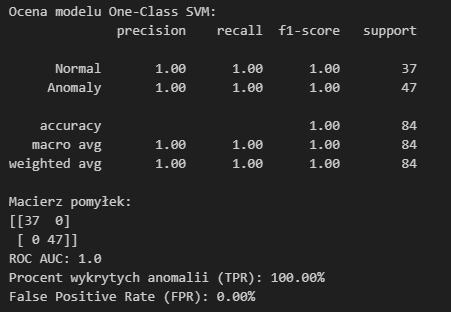
\includegraphics[scale=.70]{wykresy/ocena1.png}
	\caption{Ocena modelu One-class SVM}
	\label{FIG:1}
\end{figure}

Precision: Jest to miara, która określa, jaki odsetek przypadków oznaczonych przez model jako „Anomaly” rzeczywiście jest anomaliami. W tym przypadku precyzja dla obu klas (Normal i Anomaly) wynosi 1.00 (100\%), co oznacza, że wszystkie przypadki zaklasyfikowane jako „Normal” i „Anomaly” przez model są poprawne.

Recall: Jest to miara, która określa, jaki odsetek rzeczywistych przypadków „Anomaly” został poprawnie wykryty przez model. Wartość 1.00 dla obu klas oznacza, że model poprawnie rozpoznał 100\% przypadków normalnych i anomalnych.

F1-Score: To średnia harmoniczna precyzji i czułości, która jest przydatna w sytuacjach, gdzie istnieje nierównowaga między klasami (np. liczba przypadków normalnych i anomalnych). Wartość F1-Score 1.00 oznacza, że model jest bardzo dobrze zbalansowany i radzi sobie perfekcyjnie w wykrywaniu obu klas.

Support: To liczba przypadków w każdej klasie (37 przypadków normalnych i 47 anomalii).

Accuracy: Całkowita dokładność modelu (accuracy) to 100\%, co oznacza, że model poprawnie sklasyfikował wszystkie 84 przypadki testowe (37 normalnych i 47 anomalnych).

Macierz pomyłek:
[[37, 0],
 [ 0, 47]]
Macierz ta pokazuje, że wszystkie 37 przypadków normalnych zostały poprawnie sklasyfikowane jako normalne, a wszystkie 47 anomalii zostały poprawnie oznaczone jako anomalie. Brak błędnych klasyfikacji (nie ma wartości poza główną przekątną), co wskazuje na perfekcyjne działanie modelu.

ROC AUC (Area Under the Curve):  wynosi 1.0, co oznacza idealną zdolność modelu do rozróżniania między klasami „Normal” i „Anomaly”. Wartość 1.0 w AUC oznacza, że model jest perfekcyjny, a jego wyniki są w 100\% poprawne.

Procent wykrytych anomalii (True Positive Rate, TPR): Procent wykrytych anomalii wynosi 100\%. TPR, czyli odsetek rzeczywistych anomalii, które zostały poprawnie oznaczone jako anomalie, wynosi 100\%. Model wykrył wszystkie anomalia bez pominięcia żadnego przypadku.
False Positive Rate (FPR): FPR wynosi 0\%, co oznacza, że model nie popełnił żadnego błędu, oznaczając przypadek normalny jako anomalię. Wartość FPR 0\% oznacza, że model idealnie oddzielił przypadki normalne od anomalii bez żadnych fałszywych alarmów.


\subsection{Wynik analizy (wykresy znajdują się na końcu opracowania)}

Opis wykresów

\section{Opis wyników}


\section{Podsumowanie}


\section{Bibliografia}

[1] https://diag.pl/pacjent/artykuly/jakie-sa-pierwsze-objawy-i-sposoby-leczenia-stwardnienia-rozsianego/

[2] https://www.medicover.pl/o-zdrowiu/stwardnienie-rozsiane-objawy-przyczyny-i-leczenie,6619,n,192

[3] https://pl.wikipedia.org/wiki/Stwardnienie\_rozsiane

[4] https://ptsr.org.pl/strona/133,covid-19-a-sm

[5] Sormani MP, De Rossi N, Schiavetti I, Carmisciano L, Cordioli C, Radaelli M, et al. Disease modifying therapies and COVID-19 severity in multiple sclerosis. Ann Neurol. 2021 Apr

[6] Louapre C, Collongues N, Stankoff B, Giannesini C, Papeix C, Bensa C, et al. Clinical characteristics and outcomes in patients with coronavirus disease 2019 and multiple sclerosis. JAMA Neurol. 2020 Sep

[7] Simpson-Yap S, De Brouwer E, Kalincik T, Rijke N, Hillert JA, Walton C, et al. Associations of Disease-Modifying Therapies With COVID-19 Severity in Multiple Sclerosis. Neurology. 2021 Nov

[8] Schiff MA, Rae-Grant A, Gilden D, Franklin GM. Practice guideline: Disease-modifying therapies for adults with multiple sclerosis: Report of the guideline development, dissemination, and implementation subcommittee of the American Academy of Neurology. Neurology. 2019 Jan

[9] Erfani P, Mitchell AJ, Hameed S, Heydarpour P, Ghaffaripour R, Sahraian MA. Systematic review of health-related quality of life in multiple sclerosis patients: The impact of pharmacological treatments and lifestyle. J Neurol Sci. 2016 Dec

[10] Calabresi PA. Diagnosis and management of multiple sclerosis. Am Fam Physician. 2004 Nov

[11] Montgomery S, Hillert J, Bahmanyar S. Hospital admission due to infections in multiple sclerosis patients. Eur J Neurol. 2013 Aug

[12] Peeters LM, Parciak T, Walton C, Geys L, Moreau Y, De Brouwer E, et al. COVID-19 in people with multiple sclerosis: A global data sharing initiative. Mult Scler Houndmills Basingstoke Engl. 2020 Sep

[13] Simpson-Yap S, De Brouwer E, Kalincik T, Rijke N, Hillert JA, Walton C, et al. Associations of Disease-Modifying Therapies With COVID-19 Severity in Multiple Sclerosis. 
Neurology. 2021 Nov

[14] https://physionet.org/content/patient-level-data-covid-ms/1.0.1/

[15] https://www.geeksforgeeks.org/understanding-one-class-support-vector-machines/

[16] https://scikit-learn.org/dev/modules/generated/sklearn.svm.OneClassSVM.html

[17] https://www.baeldung.com/cs/one-class-svm

[18] https://medium.com/@roshmitadey/anomaly-detection-using-support-vectors-2c1b842213ed

[19] https://github.com/przemyslawJura00/RozpoznawanieWzorcowGrupa4




\newpage
\newpage
\begin{figure}[h]
	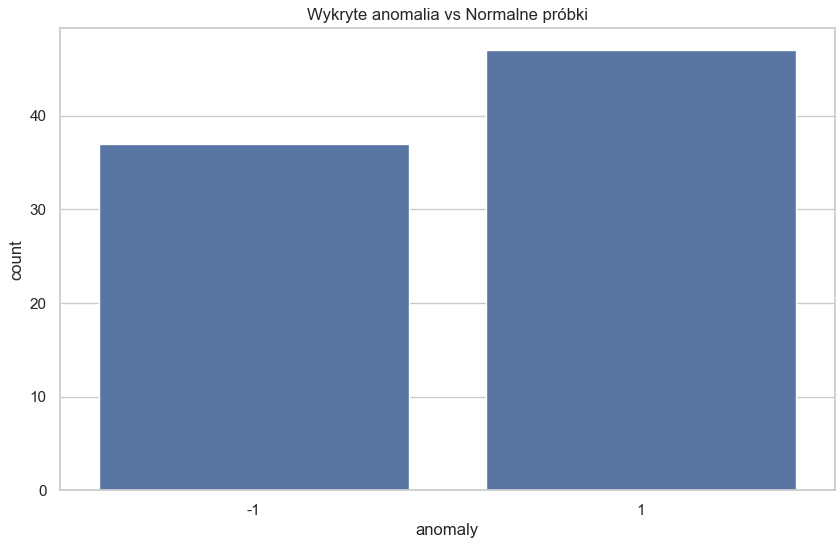
\includegraphics[scale=.40]{wykresy/wykres1.png}
	\caption{Wykryte anomalia vs Normalne próbki: -1: anomalia 1: normalny przypadek}
	\label{FIG:1}
\end{figure}

\begin{figure}[h]
	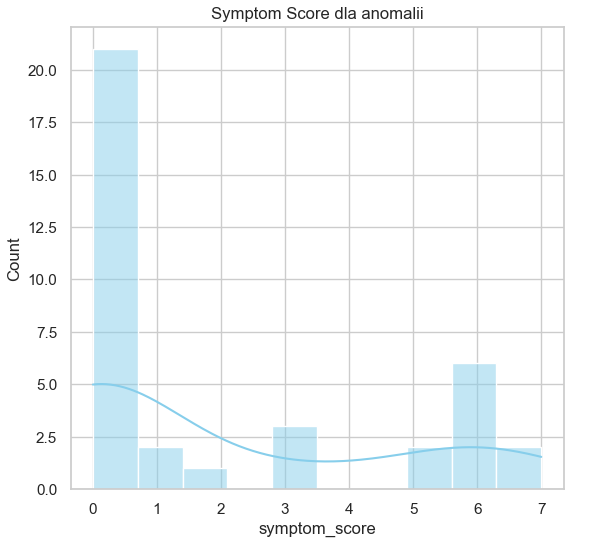
\includegraphics[scale=.73]{wykresy/wykres2.1.png}
	\caption{Rozkład ilości symptomów dla anomalii}
	\label{FIG:1}
\end{figure}

\begin{figure}[h]
	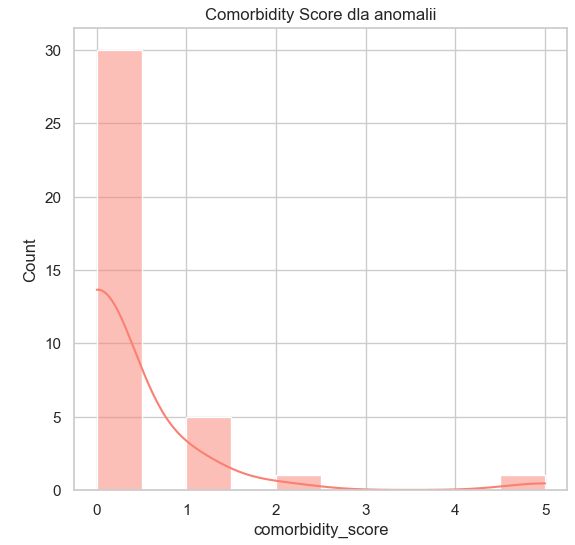
\includegraphics[scale=.73]{wykresy/wykres2.2.png}
	\caption{ Rozkład ilości chorób wspóistniejących dla anomalii}
	\label{FIG:1}
\end{figure}

\begin{figure}[h]
	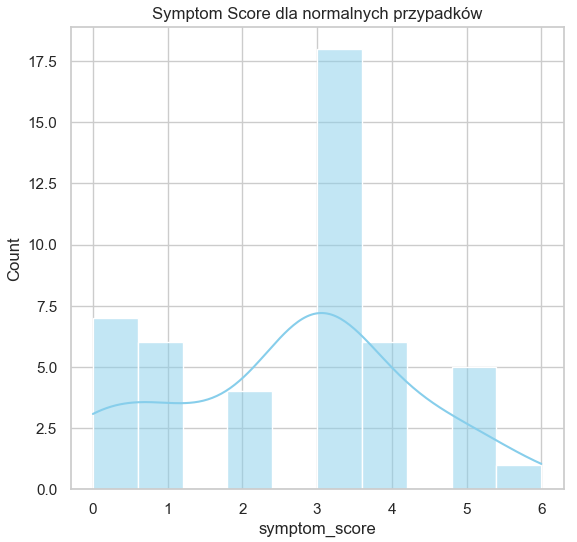
\includegraphics[scale=.73]{wykresy/wykres3.1.png}
	\caption{Rozkład ilości symptomów dla przypadków normalnych}
	\label{FIG:1}
\end{figure}

\begin{figure}[h]
	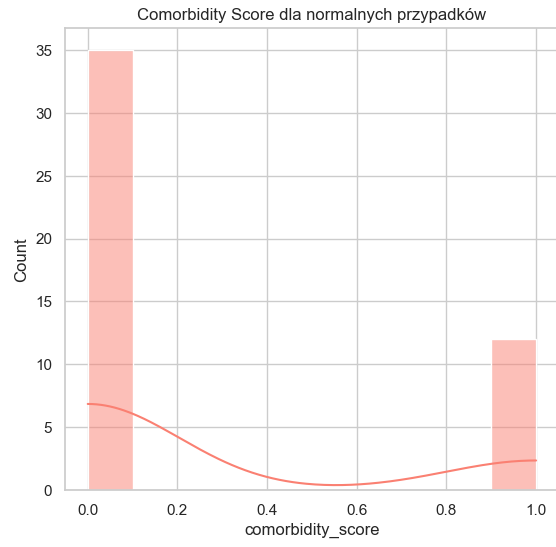
\includegraphics[scale=.73]{wykresy/wykres3.2.png}
	\caption{Rozkład ilości chorób wspóistniejących dla przypadków normalnych}
	\label{FIG:1}
\end{figure}

\begin{figure}[h]
	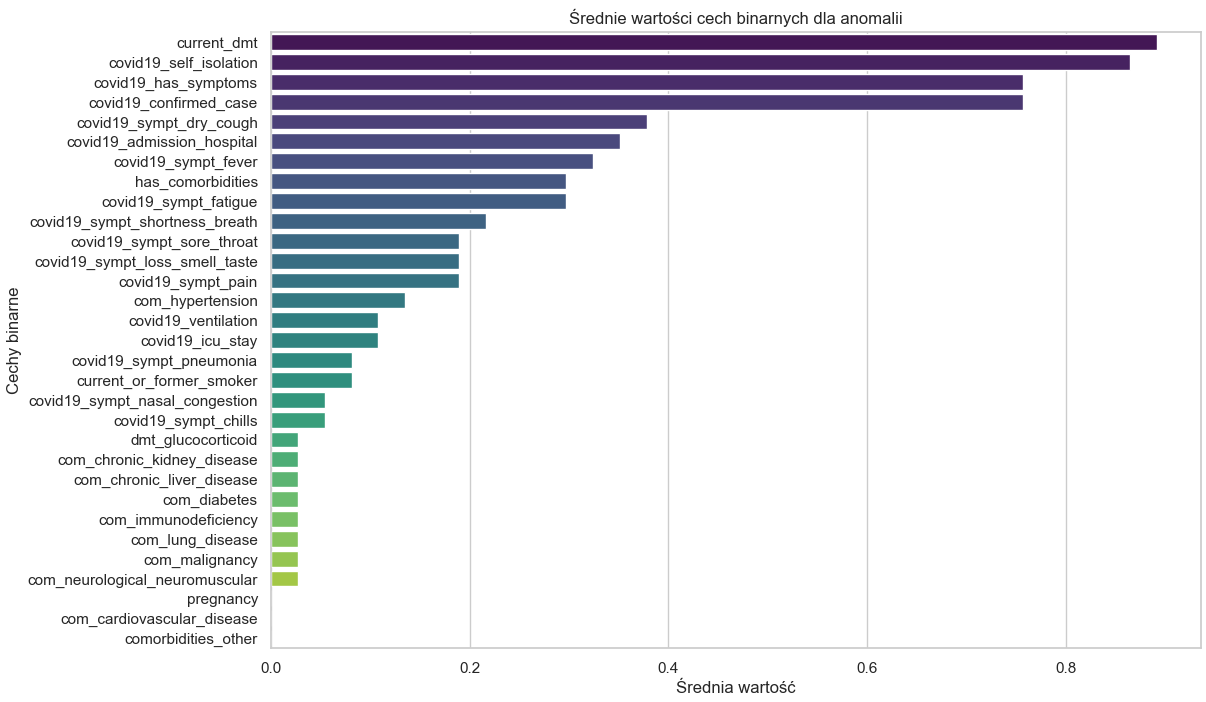
\includegraphics[scale=.35]{wykresy/wykres4.png}
	\caption{Średnie wartości charakterystycznych cech dla anomalii}
	\label{FIG:1}
\end{figure}

\begin{figure}[h]
	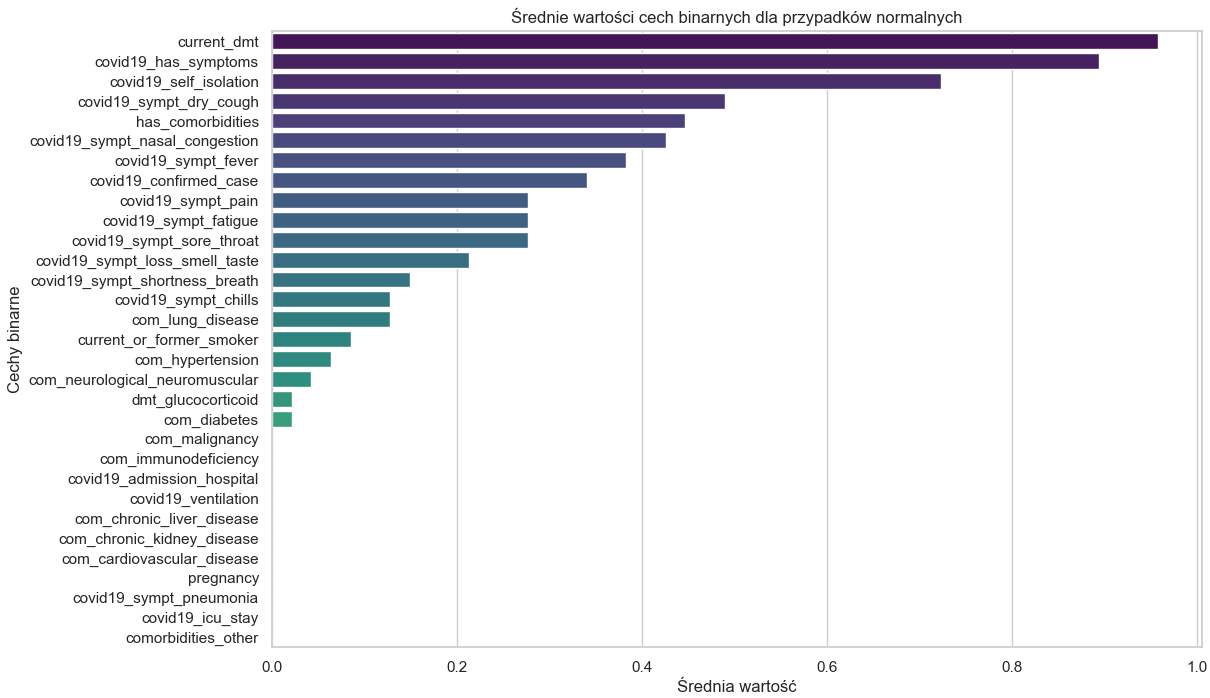
\includegraphics[scale=.35]{wykresy/wykres5.png}
	\caption{Średnie wartości charakterystycznych cech dla przypadków normalych}
	\label{FIG:1}
\end{figure}

\begin{figure}[h]
	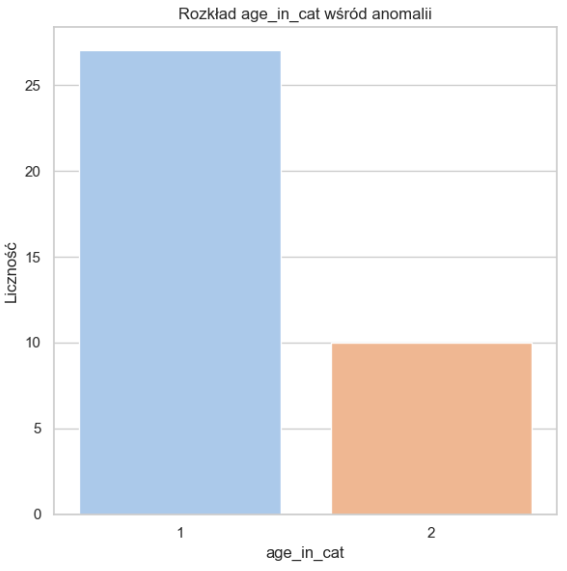
\includegraphics[scale=.73]{wykresy/wykres6.png}
	\caption{Rozkład wieku wśród anomalii: 0: jeśli zakres wieku mieści się w przedziale od 0 do <18. 
1: jeżeli przedział wiekowy mieści się w przedziale od 18 do <=50 lat.
2: jeżeli przedział wiekowy mieści się w przedziale od 51 do <=70 lat.
3: jeśli przedział wiekowy wynosi 71 lat lub więcej..}
	\label{FIG:1}
\end{figure}

\begin{figure}[h]
	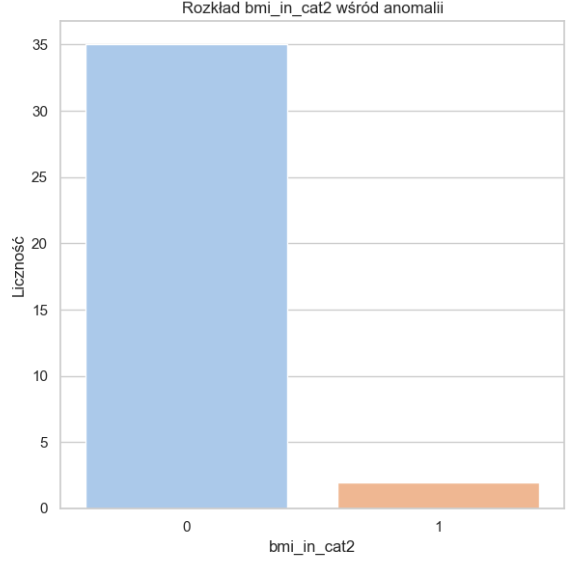
\includegraphics[scale=.73]{wykresy/wykres7.png}
	\caption{Rozkład bmi wśród anomalii: 0: not\_overweight: if BMI <= 30 kg/m2 
1: overweight: if BMI > 30 kg/m2.}
	\label{FIG:1}
\end{figure}

\begin{figure}[h]
	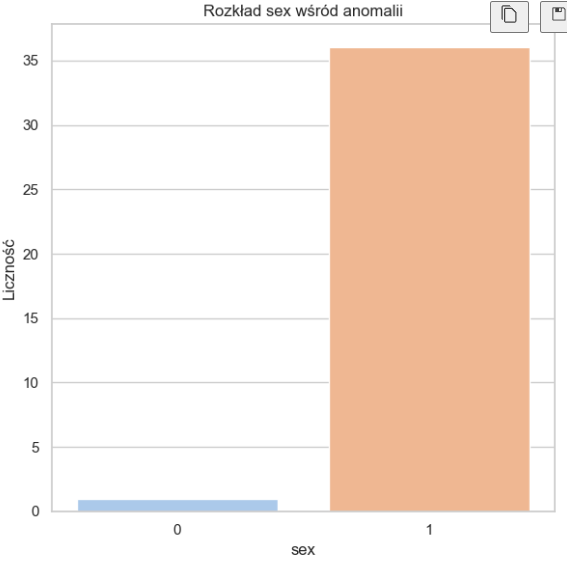
\includegraphics[scale=.73]{wykresy/wykres8.png}
	\caption{Rozkład płci wśród anomalii: 0: mężczyźni 1: kobiety}
	\label{FIG:1}
\end{figure}

\begin{figure}[h]
	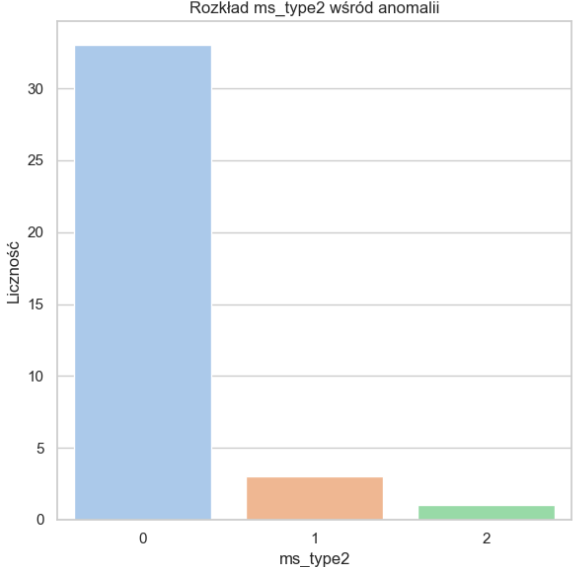
\includegraphics[scale=.73]{wykresy/wykres9.png}
	\caption{Rozkład typu stwardnienia rozsianego wśród anomalii:  0: relapsing\_remitting: jeśli typ stwardnienia rozsianego to stwardnienie rozsiane rzutowo-remisyjne (RRMS)
1: progresywny\_MS: jeśli typ stwardnienia rozsianego to wtórnie postępujące stwardnienie rozsiane (SPMS) lub pierwotnie postępujące stwardnienie rozsiane (PPMS)
2: inny: jeśli typ stwardnienia rozsianego to zespół izolowany klinicznie (CIS) lub pusty lub „niepewny”, w przypadku gdy pacjent lub lekarz nie był pewien.}
	\label{FIG:1}
\end{figure}

\begin{figure}[h]
	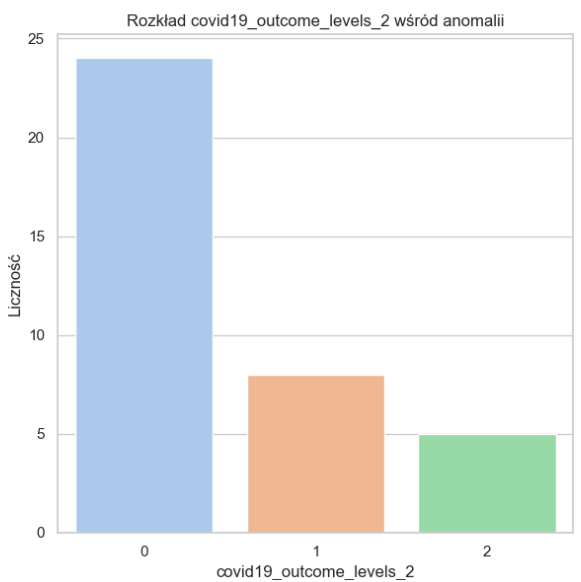
\includegraphics[scale=.73]{wykresy/wykres10.png}
	\caption{Rozkład hospitalizowanych przypadków: 0: Jeśli dana osoba ma Covid-19, ale nie była hospitalizowana.
1: Osoba ma Covid-19 i została hospitalizowana.
2: Osoba ma Covid-19, była hospitalizowana, przebywała na oddziale intensywnej terapii i/lub przebywała w ośrodku wentylacyjnym.
3: Osoba zmarła z powodu Covid-19 (nieobecna w tym zbiorze danych).}
	\label{FIG:1}
\end{figure}




\end{document}

